\documentclass{article}
\usepackage{tikz}
\usetikzlibrary{shapes.geometric,positioning}

\begin{document}
\section{Prolog}
\begin{figure}
\centering
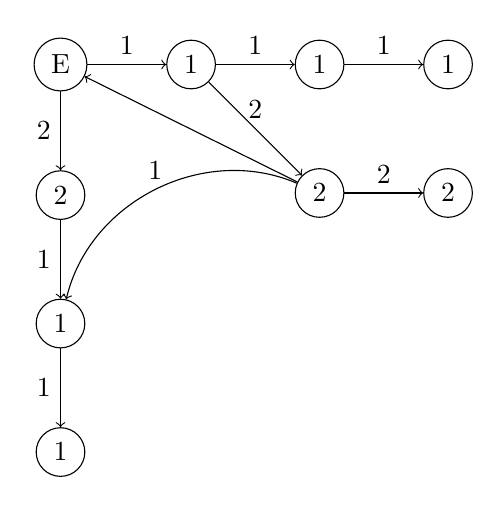
\begin{tikzpicture}[node/.style={draw,circle}]
\coordinate (origin)  at (0, 0);
\node[node] at (origin) (entry) {E};

\node[node, right=of entry] (s1e) {1};
\node[node, right=of s1e] (s11) {1};
\node[node, right=of s11] (s1f) {1};

\node[below=of s1e] (s2e) {};
\node[node, below=of s11] (s21) {2};
\draw[->] (s21) to (entry);

\node[node, right=of s21] (s2f) {2};

\node[node, below=of entry] (s3e) {2};
\node[node, below=of s3e] (s31) {1};

\node[node, below=of s31] (s3f) {1};
\draw[bend right=50, ->] (s21) to node[midway, above] {1} (s31);

\draw[->] (entry) -- (s1e) node[midway, above] {1};
\draw[->] (entry) -- (s3e) node[midway, left] {2};

\draw[->] (s1e) -- (s11) node[midway, above] {1};
\draw[->] (s11) -- (s1f) node[midway, above] {1};

\draw[->] (s1e) -- (s21) node[midway, above] {2};
\draw[->] (s21) -- (s2f) node[midway, above] {2};

\draw[->] (s3e) -- (s31) {} node[midway, left] {1};
\draw[->] (s31) -- (s3f) {} node[midway, left] {1} ;
\end{tikzpicture}
\caption{Base}
\end{figure}

\begin{figure}
\centering
\begin{tikzpicture}[node/.style={draw,circle}]
\coordinate (origin)  at (0, 0);
\node[node] at (origin) (entry) {E};
\draw[loop, ->] (entry) to node[midway, above] {0} (entry);

\node[node, right=of entry] (s1e) {1};
\draw[bend right=50, ->] (s1e) to node[midway, above] {0} (entry);

\node[node, right=of s1e] (s11) {1};
\draw[bend right=65, ->] (s11) to node[midway, above] {0} (entry);
\coordinate[above=of entry] (b1);
\draw[bend right=50, ->] (s11) to (b1) to node[midway, left] {2} (s3e);

\node[node, right=of s11] (s1f) {1};
\draw[out=100, in=90, ->] (s1f) to node[midway, above] {0} (entry);
\coordinate[above left=of b1] (b2);
\draw[bend right=60, ->] (s1f) to (b2) to node[midway, left] {2} (s3e);
\draw[loop right, ->] (s1f) to node[midway, right] {1} (s1f);

\node[below=of s1e] (s2e) {};
\node[node, below=of s11] (s21) {2};
\draw[bend left=50, ->] (s21) to node[midway, above] {1} (s31);
\draw[bend left=20, ->] (s21) to node[midway, above] {0} (entry);

\node[node, right=of s21] (s2f) {2};
\draw[bend left=50, ->] (s2f) to node[midway, above] {2} (s3e);
\draw[bend left=50, ->] (s2f) to node[midway, above] {1} (s31);
\draw[bend left=50, ->] (s2f) to node[midway, above] {0} (entry);


\node[node, below=of entry] (s3e) {2};
\draw[loop right, ->] (s3e) to node[midway, above] {2} (s3e);
\draw[bend left=50, ->] (s3e) to node[midway, left] {0} (entry);

\node[node, below=of s3e] (s31) {1};
\draw[bend left=50, ->] (s31) to node[midway, below] {2} (s21);
\draw[bend left=50, ->] (s31) to node[midway, left] {0} (entry);

\node[node, below=of s31] (s3f) {1};
\draw[loop right, ->] (s3f) to node[midway, right] {2} (s2f);
\draw[loop left, ->] (s3f) to node[midway, left] {1} (s2f);
\draw[loop below=50, ->] (s3f) to node[midway, below] {0} (s2f);

\draw[->] (entry) -- (s1e) node[midway, above] {1};
\draw[->] (entry) -- (s3e) node[midway, left] {2};

\draw[->] (s1e) -- (s11) node[midway, above] {1};
\draw[->] (s11) -- (s1f) node[midway, above] {1};

\draw[->] (s1e) -- (s21) node[midway, above] {2};
\draw[->] (s21) -- (s2f) node[midway, above] {2};

\draw[->] (s3e) -- (s31) {} node[midway, left] {1};
\draw[->] (s31) -- (s3f) {} node[midway, left] {1} ;
\end{tikzpicture}
\caption{Base}
\end{figure}


\section{REGEX}
% ^(0|1|20|22|212|210)*(111|122)\$
111
1112
1122
122
2111
00121222
00120122
001211222
01201201111
01201202111

% \bibliographystyle{plain} % We choose the "plain" reference style
% \bibliography{refs}
\end{document}